\documentclass{ctexart}
\usepackage{graphicx}
\usepackage{amsmath}
\usepackage{amssymb}
\usepackage{hyperref}
\usepackage{geometry}
\usepackage{enumitem}
\usepackage{booktabs}
\usepackage{array}
\geometry{a4paper, left=1in, right=1in, top=1in, bottom=1in}

\title{《深度学习基础》课程大作业报告}
\author{PB24000056 胡家硕\quad PB24000150 李欣宸\quad PB24000384 张谋琪}
\date{\today}

\begin{document}

\maketitle

本文是《深度学习基础》课程大作业报告。代码主体位于 \verb|code/|，最终模拟交易使用的模型、数据和信号生成脚本保存在
\verb|experiments/final_competition_package_20260601/|；其中 \verb|FINAL_RUNBOOK.md| 记录了最终使用的模型和交易流程。报告包含数据处理、问题定义、模型训练、历史回测、模拟交易和总结反思。真实比赛收益截图、最终成绩截图和组员具体分工中无法从代码判断的部分在文中以“待补充”标出。

\section{实验设置}

\paragraph{股票池与数据来源}
本实验使用沪深 300 作为股票池（而不是全 A 股）。这样做的主要原因是：沪深 300 成分股流动性较好，停牌、极端异常和小盘股噪声相对少；同时 300 只左右股票已经足够构造横截面排序任务，便于在有限训练时间内完成模型对比和回测。最终面板中实际可用股票为 299 只。直接原因是成分股文件中中航成飞写作 \verb|302132|，而原始数据和基础信息表中写作 \verb|302132.SZ|；代码中的股票代码规范化函数没有把 \verb|302| 前缀自动识别为深交所代码，因此过滤股票池时未能匹配这一只股票。这个问题只影响股票池覆盖数量，不影响剩余 299 只股票上的训练、验证和回测流程。

使用的数据包括三类：基础日频量价数据、每日基本面/估值指标和每日资金流向数据。主面板文件名为 \verb|panel_hs300_advanced.npz|；最终比赛包中使用同名副本，具体路径见 \verb|FINAL_RUNBOOK.md|。

\paragraph{特征工程}
模型输入为过去 30 个交易日的特征序列。特征共 40 维，主要分为三类：
\begin{itemize}[noitemsep]
    \item 量价特征：1/5/20 日收益率、5/20 日乖离率、20 日波动率、MACD 比例、RSI、振幅、成交量和成交额变化等；
    \item 基本面特征：换手率、市盈率倒数、市净率倒数、市销率倒数、股息率、市值和股本规模等；
    \item 资金流特征：净流入金额比例、主力资金比例、大单/中单/小单净流入比例，以及 3 日和 5 日平滑资金流特征。
\end{itemize}

这些特征均由 \verb|load_data.py| 构造。对于不同量纲的特征，代码按交易日做横截面 winsorized z-score 标准化：对同一天所有股票计算均值和标准差，先进行 3 倍标准差截尾，再转为 z-score。这样不会使用未来日期的数据统计量，也更符合横截面选股任务。特征构造的具体思路在第 \ref{sec:analysis} 节中展开。

\paragraph{标签与时间对齐}
由于比赛数据在盘后更新，若在交易日 $t$ 收盘后生成信号，实际只能在 $t+1$ 日开盘执行。因此标签没有使用 $t$ 到 $t+1$ 的收盘收益，而是使用 open-to-open 收益：
\[
    r_t = \frac{\mathrm{open}_{t+2}}{\mathrm{open}_{t+1}} - 1 .
\]
这对应“用 $t$ 日及以前的特征，在 $t+1$ 日开盘买入，并持有到 $t+2$ 日开盘”。最终比赛模型进一步使用未来 3 日 open-to-open 复合收益作为训练标签，即 \verb|label_horizon=3|。这样做牺牲了一部分短期灵敏度，但可以降低单日收益噪声，使模型更偏向选择短期趋势更稳定的股票。

\paragraph{数据划分}
训练集为 2016-01-04 至 2025-12-31，验证集为 2026-01-01 至 2026-02-27，样本外评估主要使用 2026 年 3 月以后的数据。划分完全按日期完成，以避免时间序列任务中的信息泄露。

\section{模型与训练方法}

\subsection{模型结构}

最终使用的模型是 Transformer 横截面股票打分模型。输入张量形状为
\[
    (B, N, T, F),
\]
其中 $B$ 为 batch size，$N$ 为股票数，$T=30$ 为时间窗口长度，$F=40$ 为特征数。模型对每只股票共享同一套时间序列编码器，输出形状为 $(B,N)$ 的预测分数。

具体结构为：先将 40 维输入特征线性映射到 $d_{\mathrm{model}}=64$，加入正弦位置编码后输入 2 层 Transformer Encoder，每层使用 4 个注意力头，前馈层维度为 $4d_{\mathrm{model}}$，激活函数为 GELU，dropout 为 0.15。最后取序列最后一天的隐状态，通过 LayerNorm 和两层 MLP 输出单个股票分数。

模型输出股票分数。这样做其实是一种折中选择：金融任务中预测精确收益很困难，比起直接训练一个输出策略的模型，预测分数的模型需要学习的约束更少，而人工设计的交易策略为模型提供了较强的先验。我们的交易策略将在后续部分介绍。

\paragraph{训练对象与防止过拟合}
最直观地说，模型训练的不是“明天一定涨多少”，而是“在同一天的 299 只股票里，哪些股票未来几天相对更值得买”。训练样本由 30 个交易日的历史特征窗口组成，标签是之后 3 日 open-to-open 复合收益。模型看到过去 30 天的量价、估值和资金流特征，输出每只股票一个分数；训练时希望高分股票的未来收益也更高。

为了降低过拟合，训练和策略中采取了以下措施：
\begin{itemize}[noitemsep]
    \item 按日期划分训练集和验证集，不随机混合未来日期；
    \item 特征只按单日横截面标准化，不在全量时间上计算均值和方差；
    \item 使用 3 日复合收益标签，减少单日噪声对模型的影响；
    \item Transformer 规模较小，只使用 2 层、64 维隐藏层，并加入 dropout；
    \item 优化器使用 AdamW 和 weight decay，并在反向传播时做梯度裁剪；
    \item 按验证集 IC 或 Sharpe 保存 checkpoint，而不是只看训练集损失；
    \item 最终交易时不完全相信模型原始分数，而是加入趋势过滤、波动惩罚和止损规则。
\end{itemize}

\subsection{训练目标}

训练时主要优化横截面排序能力。损失函数由三部分组成：
\[
    \mathcal{L}
    = -\mathrm{IC}(s,r)
    + \alpha \cdot \mathrm{MSE}(z(s), z(r))
    - \beta \cdot \mathrm{Sharpe}(w(s), r),
\]
其中 $s$ 是模型分数，$r$ 是未来收益，$z(\cdot)$ 表示在同一交易日横截面内标准化。第一项最大化预测分数和未来收益的 Pearson IC；第二项让 z-score 后的预测分数接近 z-score 后的收益；第三项用可微的 softmax Top-$N$ 权重近似组合 Sharpe。实际代码中 $\alpha=0.1,\beta=0.05$。

这种损失比直接回归原始收益更符合任务：原始日收益噪声很大，绝对数值很难预测；但如果模型能把未来表现较好的股票排在前面，就可以通过 Top-$N$ 策略转化为交易组合。

\subsection{模型选择}

实验阶段比较了 Transformer、GRU、LSTM 和若干改进模型。表 \ref{tab:oos-results} 给出一组样本外回测结果。可以看到，基线模型在 2026 年 3 月以后的样本外区间收益均为负，而加入更长标签、趋势过滤和低频调仓的改进模型有明显改善。

\begin{table}[htbp]
\centering
\caption{样本外回测指标对比（2026-03-02 至 2026-05-27）}
\label{tab:oos-results}
\begin{tabular}{lrrrr}
\toprule
模型 & 最终收益 & Sharpe & 最大回撤 & 平均换手 \\
\midrule
Transformer & -4.41\% & -0.596 & -11.54\% & 0.607 \\
GRU & -7.27\% & -1.666 & -9.61\% & 0.597 \\
LSTM & -4.39\% & -0.802 & -8.18\% & 0.597 \\
Improved Transformer & 29.94\% & 3.325 & -9.17\% & 0.294 \\
\bottomrule
\end{tabular}
\end{table}

表中“最终收益”“Sharpe”“最大回撤”“平均换手”分别对应回测代码输出中的 \verb|final_return|、\verb|sharpe|、\verb|max_drawdown| 和 \verb|avg_turnover|。

\begin{figure}[htbp]
    \centering
    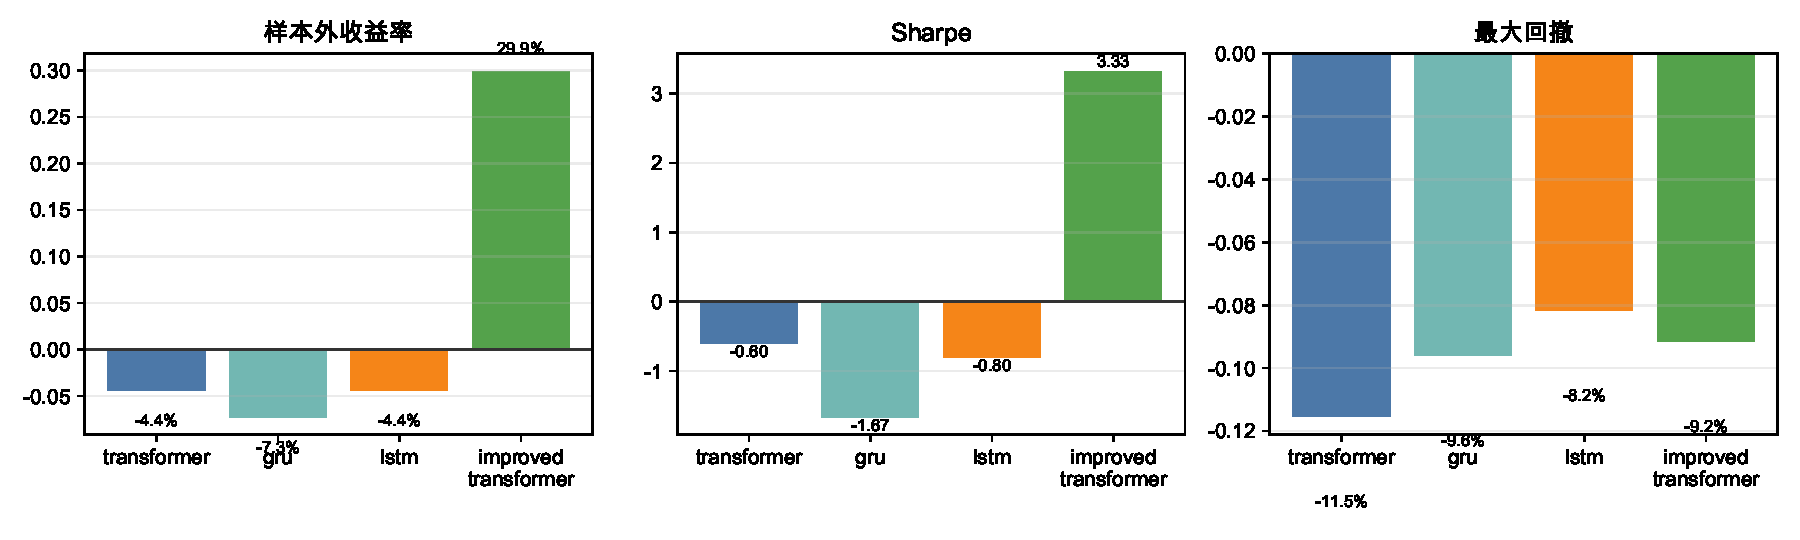
\includegraphics[width=\textwidth]{figures/model_metric_compare.pdf}
    \caption{主要模型样本外收益、Sharpe 与最大回撤对比}
    \label{fig:model-metric-compare}
\end{figure}

最终比赛使用的模型为 \verb|improved_h3_e50_best__improved__i5__slm0p035|，checkpoint 为 \verb|model/improved_h3_e50_best.pt|。该模型使用 Transformer 架构、3 日标签、50 个 epoch 训练，并在独立 10 日窗口回测中表现较稳定。它在前一个 10 日窗口平均收益为 12.17\%，正收益窗口占比为 1.0；在最近 10 日回测中收益为 22.08\%，Sharpe 为 12.48，最大回撤为 -1.92\%。

\section{交易策略与历史回测}

\subsection{交易规则}

最终交易策略不是直接使用模型分数，而是在模型分数基础上加入人工构造的交易分数：
\[
\begin{aligned}
\mathrm{trade\_score}
&= \mathrm{model\_score}
 + 0.18 \cdot \mathrm{ret\_20d}
 + 0.12 \cdot \mathrm{bias\_20} \\
&\quad + 0.06 \cdot \mathrm{main\_force\_amount\_ratio\_5d}
 - 0.10 \cdot \mathrm{volatility\_20d}.
\end{aligned}
\]
同时，买入候选需要满足
\[
    \mathrm{ret\_20d}>-0.35,\quad
    \mathrm{bias\_20}>-0.50,\quad
    \mathrm{volatility\_20d}<2.25 .
\]

这一设计是对基础作业要求中简单 ``Top $n$ / Sell $k$ / Buy $k$'' 策略的改进。模型分数负责给出横截面预测，趋势项和资金流项用于降低模型买入短期严重下跌股票的概率，波动率惩罚用于控制组合尾部风险。由于训练目标优化的是排序 IC，而不完全等同于实际组合收益和回撤，因此这里加入了少量可解释的风险控制规则。

实际组合规则如下：
\begin{itemize}[noitemsep]
    \item 持仓数量为 10，只股票等权；
    \item 初始日买入交易分数最高的 10 只股票；
    \item 每 5 个交易日进行一次主调仓，卖出当前持仓中分数较低的 3 只，并买入候选中分数较高的 3 只；
    \item 若单只股票最近已实现收益小于等于 -3.5\%，则触发止损替换；
    \item 单边交易成本按 0.0005 计入回测。
\end{itemize}

\subsection{最近 10 日回测}

最终策略在 2026-05-14 至 2026-05-27 的最近 10 个可完整回测交易日中，最终净值为 1.2208，对应收益 22.08\%。图 \ref{fig:latest10-nav} 和图 \ref{fig:latest10-ret-turnover} 给出净值、日收益和换手情况；它们在回测输出中对应 \verb|nav|、\verb|net_ret| 和 \verb|turnover|。

\begin{figure}[htbp]
    \centering
    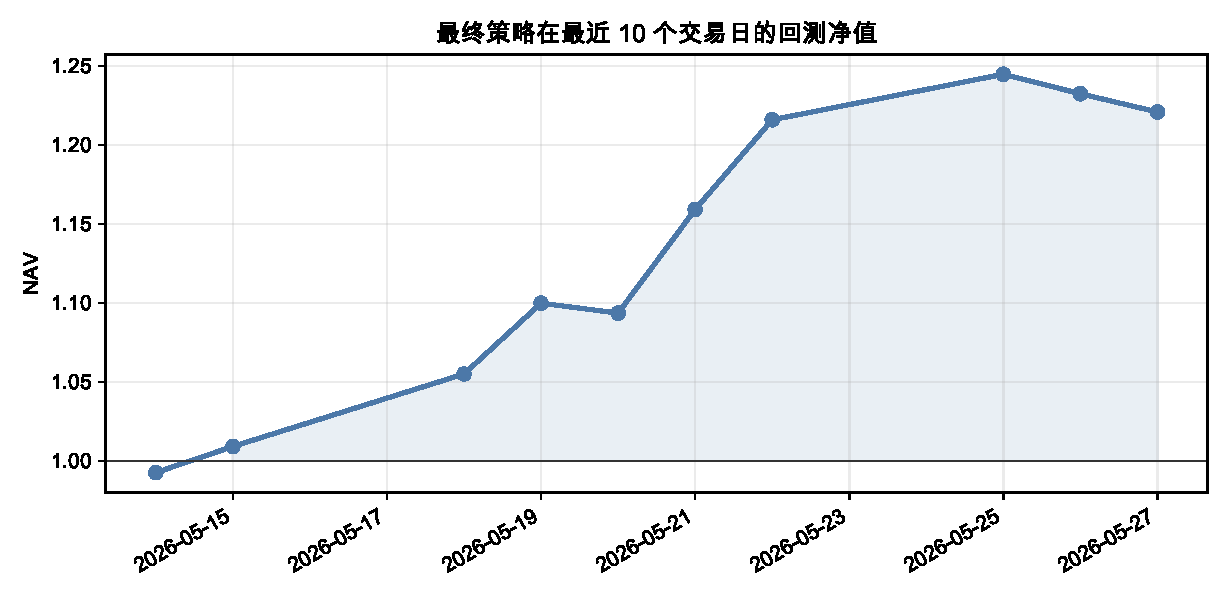
\includegraphics[width=0.9\textwidth]{figures/final_strategy_latest10_nav.pdf}
    \caption{最终策略最近 10 个交易日回测净值}
    \label{fig:latest10-nav}
\end{figure}

\begin{figure}[htbp]
    \centering
    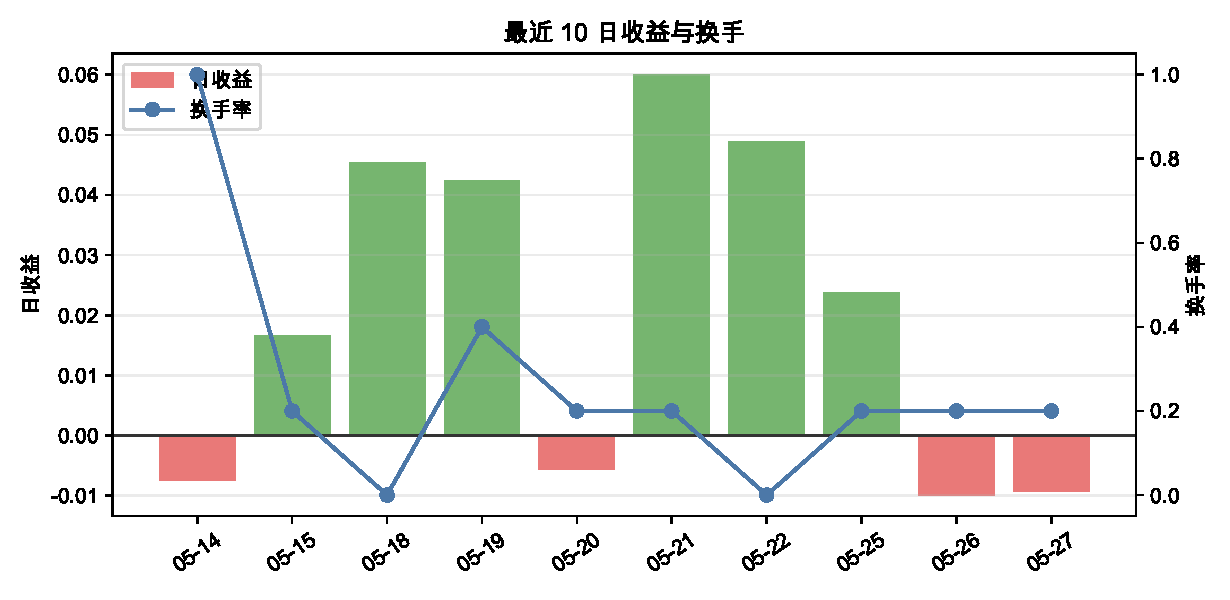
\includegraphics[width=0.9\textwidth]{figures/final_strategy_latest10_ret_turnover.pdf}
    \caption{最终策略最近 10 日收益与换手}
    \label{fig:latest10-ret-turnover}
\end{figure}

该回测窗口表现较好，但不能简单视为未来收益的保证。原因有三点：首先，10 个交易日样本很短，容易受到行情风格影响；其次，沪深 300 中电子、半导体等行业在该窗口表现较强，而最终模型初始持仓中这类股票占比较高；最后，策略中仍然有人工调整的趋势过滤和止损规则，它们改善了该阶段回测，但也可能在震荡市场中错过反转机会。

\section{模拟交易}

\subsection{比赛执行流程}

正式比赛时间为 2026-06-01 至 2026-06-12，共 10 个交易日。最终比赛包中已经将每日交易序号、数据刷新和信号生成流程写入 \verb|FINAL_RUNBOOK.md|。实际执行时，每个交易日盘后先更新数据并重建面板，再运行 \verb|live_trade_signal.py| 生成下一交易日的目标持仓和买卖订单。

比赛日历如表 \ref{tab:competition-calendar} 所示。周末不运行信号，也不增加交易序号。

\begin{table}[htbp]
\centering
\caption{模拟交易比赛日历}
\label{tab:competition-calendar}
\begin{tabular}{ccl}
\toprule
交易序号 & 日期 & 操作 \\
\midrule
1 & 2026-06-01 & 初始建仓 \\
2 & 2026-06-02 & 日常检查 \\
3 & 2026-06-03 & 日常检查 \\
4 & 2026-06-04 & 日常检查 \\
5 & 2026-06-05 & 日常检查 \\
6 & 2026-06-08 & 5 日主调仓，Buy3/Sell3 \\
7 & 2026-06-09 & 日常检查 \\
8 & 2026-06-10 & 日常检查 \\
9 & 2026-06-11 & 日常检查 \\
10 & 2026-06-12 & 日常检查/比赛结束 \\
\bottomrule
\end{tabular}
\end{table}

\begin{figure}[htbp]
    \centering
    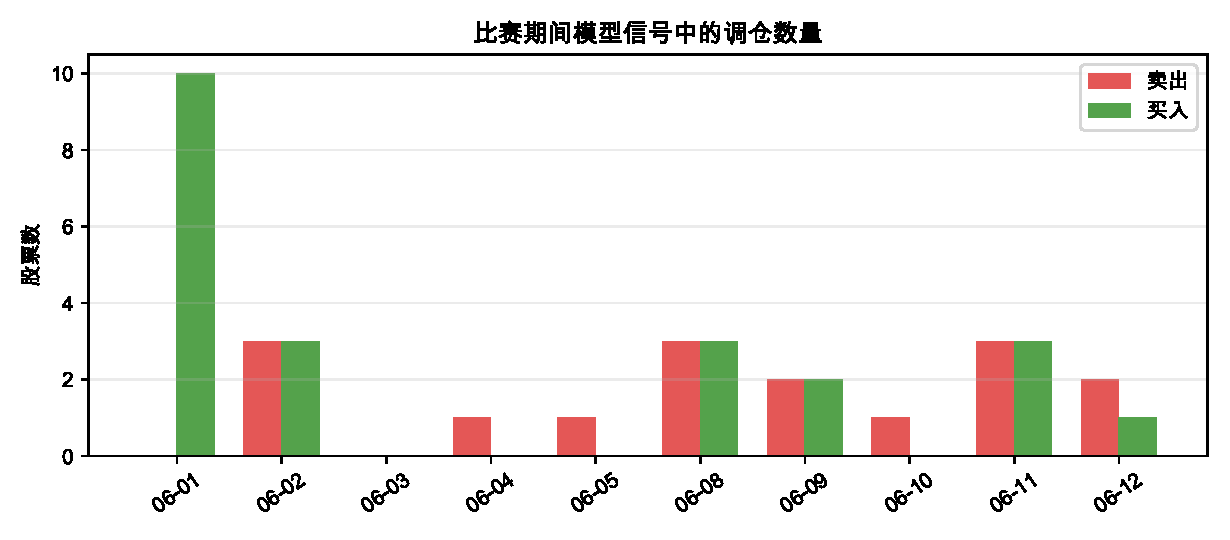
\includegraphics[width=0.9\textwidth]{figures/competition_signal_orders.pdf}
    \caption{比赛期间模型信号给出的买卖数量}
    \label{fig:competition-orders}
\end{figure}

\subsection{实盘信号与下单记录}

6 月 1 日初始建仓使用 2026-05-29 的最新数据，目标持仓为：
\[
\begin{gathered}
\texttt{300274.SZ},\ \texttt{300308.SZ},\ \texttt{300394.SZ},\ \texttt{300408.SZ},\ \texttt{300433.SZ},\\
\texttt{300661.SZ},\ \texttt{600460.SH},\ \texttt{600584.SH},\ \texttt{603986.SH},\ \texttt{688082.SH}.
\end{gathered}
\]
随后每日读取当前持仓和必要的已实现收益文件。若不是主调仓日，脚本只处理止损或无效持仓；6 月 8 日作为第 6 个交易日触发主调仓，实际信号建议卖出 \verb|600027.SH|、\verb|600584.SH|、\verb|688082.SH|，买入 \verb|000725.SZ|、\verb|000983.SZ|、\verb|600183.SH|。

需要注意的是，代码中的信号是理论目标持仓，真实模拟交易还受到 T+1、下单价格、成交情况和满仓要求影响。因此实际交易记录与模型信号存在一些出入。原始同花顺记录是一张较长的手机截图，不适合直接放入报告；这里将其中的成交记录整理为表 \ref{tab:actual-trades}。

\begin{table}[htbp]
\centering
\caption{模拟交易中的实际成交记录摘要}
\label{tab:actual-trades}
\small
\begin{tabular}{p{0.12\textwidth}p{0.38\textwidth}p{0.38\textwidth}}
\toprule
日期 & 买入 & 卖出 \\
\midrule
06-01 & 盛美上海 450 股@226.50；兆易创新 200 股@467.01；圣邦股份 900 股@115.92；天孚通信 200 股@455.16；长电科技 1200 股@80.10；阳光电源 600 股@177.91；蓝思科技 2400 股@40.50；三环集团 800 股@125.00；士兰微 2400 股@34.17；中际旭创 100 股@1161.00 & -- \\
06-02 & 华电国际 16700 股@5.58；华能国际 9800 股@9.15 & 圣邦股份 900 股@103.50；士兰微 2400 股@33.01 \\
06-05 & 士兰微 2800 股@34.98；新易盛 100 股@801.13 & 阳光电源 600 股@158.23；华能国际 9800 股@8.52 \\
06-08 & 山西焦煤 11900 股@8.01；京东方 A 15000 股@6.42；生益科技 700 股@130.47 & 盛美上海 450 股@246.50；长电科技 1200 股@72.30；华电国际 16700 股@5.11 \\
06-09 & 中国神华 1900 股@48.86；陕西煤业 3100 股@27.31 & 士兰微 2800 股@33.83；天孚通信 200 股@436.00 \\
06-11 & -- & 蓝思科技 2400 股@42.88 \\
06-12 & 长电科技 1000 股@71.50；巨化股份 2500 股@41.97；士兰微 3100 股@33.93 & 新易盛 140 股@520.00；三环集团 800 股@129.13 \\
\bottomrule
\end{tabular}
\end{table}

可以看到，实际操作总体仍然遵循模型信号的方向：6 月 1 日完成初始建仓，6 月 8 日附近执行主调仓，后续继续做止损、补仓和持仓修正。但实际成交不等于理论订单。比如某些委托无法按预期成交时，需要调整价格或用可成交股票补足仓位；当实际成交数量与理论等权数量不完全一致时，最终持仓也会和模型输出略有差别。这个差异是模拟交易中必须单独说明的部分，否则容易把“回测订单”和“真实成交”混为一谈。

\paragraph{真实比赛结果}
待补充：同花顺比赛最终收益率、收益趋势截图和最终成绩截图。

\section{结果分析与反思} \label{sec:analysis}

\subsection{特征构造思路}

本实验的特征不是简单堆字段，而是围绕“短期收益排序”这个目标构造。量价特征主要回答“这只股票最近是强还是弱”：\verb|ret_1d|、\verb|ret_5d|、\verb|ret_20d| 描述短中期收益，\verb|bias_5|、\verb|bias_20| 描述价格相对均线的位置，\verb|macd_pct| 和 \verb|rsi_14| 描述动量状态。风险特征主要回答“这个信号是否太不稳定”：\verb|volatility_20d|、振幅和日内涨跌幅可以让模型识别高波动股票。

基本面特征用于补充价格形态没有覆盖的信息。代码没有直接使用 PE/PB/PS 的原始值，而是构造 \verb|ep_ttm|、\verb|bp|、\verb|sp_ttm|，即估值指标的倒数；这样数值方向更接近“收益率”或“价值暴露”，也能减少极端 PE 的影响。市值、股本等规模变量统一取 \verb|log1p|，避免少数大市值股票支配尺度。

资金流特征用于刻画交易行为。代码将净流入金额、主力资金、大单/中单/小单净流入都除以当日成交额或成交量，得到相对强度；再构造 3 日、5 日平滑项，减少单日资金流噪声。这个设计的直觉是：如果模型只看价格，很容易把“大跌后的低位”误认为机会；加入资金流后，可以区分“有资金承接的调整”和“持续流出的下跌”。

\subsection{模型演进与问题修正}

从历史回测看，基线深度学习模型并没有稳定取得正收益。图 \ref{fig:model-metric-compare} 中，基线 Transformer、GRU、LSTM 在 2026 年 3 月以后的样本外收益分别为 -4.41\%、-7.27\% 和 -4.39\%，最大回撤也不小。这说明单纯换模型结构不能直接解决金融时间序列的噪声问题。

早期模型的一个突出问题是：它经常给近期大跌的股票较高分数，相当于在赌这些股票马上反弹。这个现象在回测中并不稳定。在最近 10 日窗口中，一些基线模型仍然排在改进模型之后，例如 \verb|transformer_best| 收益约 -0.95\%，旧的 \verb|best__baseline| 收益约 -3.62\%，而最终使用的 \verb|improved_h3_e50_best| 收益为 22.08\%。

我们推测这一现象有几个原因。第一，单日收益标签噪声很大，某些短期反转样本会让模型学到“跌得多可能会涨”的模式，但这种模式并不总是成立。第二，IC 损失只关心同一天股票排序的相关性，并不直接约束组合回撤；如果模型把少数高波动股票排在前面，IC 可能短期不差，但组合风险会很高。第三，早期每日 Sell3/Buy3 的调仓方式换手较高，如果频繁买入下跌反弹股，交易成本和错误反转会被放大。

围绕这个问题，我们尝试了多种模型结构和策略约束：模型结构上比较了 Transformer、GRU、LSTM；标签上比较了 1 日、3 日、5 日、10 日等预测窗口；策略上加入趋势过滤、波动惩罚、资金流修正、5 日主调仓和 -3.5\% 止损。最终模型采用 3 日标签的 Transformer，并在交易时不直接使用模型原始分数，而是使用包含 \verb|ret_20d|、\verb|bias_20|、\verb|main_force_amount_ratio_5d| 和 \verb|volatility_20d| 的 \verb|trade_score|。

因此，最终策略不是单纯“相信 Transformer”，而是把深度学习模型作为横截面排序器，再用趋势、波动、资金流和止损约束修正其在金融噪声下的偏差。图 \ref{fig:latest10-nav} 和图 \ref{fig:latest10-ret-turnover} 展示了最终策略在最近 10 日窗口中的净值、日收益与换手变化，可以看到收益主要来自几个强势交易日，同时换手率低于基线模型。

\subsection{收益与局限}

从收益率拆解看，最终策略最近 10 日中有 6 天为正收益，最大单日净收益出现在 2026-05-21，约为 6.00\%；最大单日净亏损出现在 2026-05-26，约为 -0.99\%。这说明收益并不是每天平滑积累，而是由少数强势交易日贡献较多。与之相比，基线模型在同一时期的平均换手约为 0.64，最终策略平均换手约为 0.26，说明 5 日主调仓确实降低了交易频率。低换手并不一定提高收益，但在 10 日比赛这种短周期场景中，它减少了无效调仓和手续费损耗，也降低了频繁追逐大跌反弹股的风险。

但改进策略也有局限。首先，趋势过滤和波动惩罚是人工规则，可能提高了近期回测表现，但不一定适用于所有市场状态。其次，沪深 300 股票池流动性较好但行业分布并不均匀，模型在某些窗口可能集中买入电子、半导体等高弹性行业，收益和回撤都容易被行业行情主导。最后，真实比赛只有 10 个交易日，收益结果受偶然性影响很大，因此本实验更重要的部分是保证数据无泄露、训练流程完整、回测规则与实盘执行尽量一致。

\section{结论}

本实验完成了从数据处理、深度学习建模、历史回测到模拟交易执行的完整流程。最终方案使用沪深 300 股票池，构造 40 维日频特征和 30 日输入窗口，训练 Transformer 模型输出横截面股票分数，并结合趋势、资金流、波动率和止损规则构造 Top10 等权组合。

主要结论如下：
\begin{itemize}[noitemsep]
    \item open-to-open 标签与盘后数据更新时间一致，可以避免在交易信号中使用未来信息；
    \item 直接优化短期收益回归并不稳定，横截面 IC 与组合 Sharpe 结合更适合选股排序任务；
    \item 基线 Transformer/GRU/LSTM 在样本外回测中表现一般，说明模型结构本身不是决定收益的唯一因素；
    \item 最终改进策略通过 3 日标签、趋势过滤、资金流修正、波动惩罚和低频调仓改善了近期回测表现；
    \item 模拟交易中需要额外考虑 T+1、成交价格、满仓约束和止损执行，这些约束使实盘结果可能偏离理论回测。
\end{itemize}

\section{提交要求对照}

根据作业提交内容要求，本报告和代码覆盖情况如下：

\begin{table}[htbp]
\centering
\caption{提交要求覆盖情况}
\label{tab:requirement-check}
\begin{tabular}{p{0.28\textwidth}p{0.62\textwidth}}
\toprule
要求 & 本报告中的对应内容 \\
\midrule
数据预处理规范 & 股票池、特征工程、横截面标准化、缺失值和 mask 处理见第 1 节。 \\
标签和任务定义合理 & open-to-open 标签、3 日复合收益标签和横截面排序任务见第 1 节。 \\
数据集划分正确 & 训练、验证、样本外回测均按日期划分，见第 1 节。 \\
无数据泄露 & 特征只使用 $t$ 日及以前数据，标准化不使用未来日期统计量，见第 1 节。 \\
模型架构设计 & Transformer 打分模型结构见第 2 节。 \\
训练流程完整 & 损失函数、训练目标、防止过拟合措施和 checkpoint 选择见第 2 节。 \\
训练有效、损失收敛 & 报告引用验证 IC、Sharpe 和回测指标；训练曲线图片可继续从实验目录补充。 \\
历史回测指标 & 年化收益、Sharpe、最大回撤、胜率、换手和最近 10 日 NAV 见第 2、3 节。 \\
结果分析和对比 & 基线模型、改进模型和“大跌股反转”问题分析见第 2、3、5 节。 \\
模拟交易流程 & 比赛日历、信号生成、实际成交记录和理论信号偏差说明见第 4 节。 \\
模拟交易收益与截图 & 实际成交记录已转写；最终收益趋势和成绩截图仍需待补充。 \\
组员姓名、学号和分工 & 姓名和学号已在标题页，具体分工仍需待补充。 \\
\bottomrule
\end{tabular}
\end{table}

\section{组员分工}

待补充。建议按照实际情况填写，例如：
\begin{itemize}[noitemsep]
    \item PB24000056 胡家硕：待补充；
    \item PB24000150 李欣宸：待补充；
    \item PB24000384 张谋琪：待补充。
\end{itemize}

\end{document}
